% B1 code-capacity content-LER vs p -- decoder ladder L1-L4.
% Auto-generated by plot_ladder_ler.py -- do not edit by hand.
%
% In your document preamble:
%     \usepackage{pgfplots}
%     \pgfplotsset{compat=1.18}
% then in the body:
%     % B1 code-capacity content-LER vs p -- decoder ladder L1-L4.
% Auto-generated by plot_ladder_ler.py -- do not edit by hand.
%
% In your document preamble:
%     \usepackage{pgfplots}
%     \pgfplotsset{compat=1.18}
% then in the body:
%     % B1 code-capacity content-LER vs p -- decoder ladder L1-L4.
% Auto-generated by plot_ladder_ler.py -- do not edit by hand.
%
% In your document preamble:
%     \usepackage{pgfplots}
%     \pgfplotsset{compat=1.18}
% then in the body:
%     % B1 code-capacity content-LER vs p -- decoder ladder L1-L4.
% Auto-generated by plot_ladder_ler.py -- do not edit by hand.
%
% In your document preamble:
%     \usepackage{pgfplots}
%     \pgfplotsset{compat=1.18}
% then in the body:
%     \input{b1_ladder_ler_vs_p.tex}
%
% Or compile this file on its own with:
%     \documentclass{standalone}
%     \usepackage{pgfplots}\pgfplotsset{compat=1.18}
%     \begin{document}\input{b1_ladder_ler_vs_p.tex}\end{document}
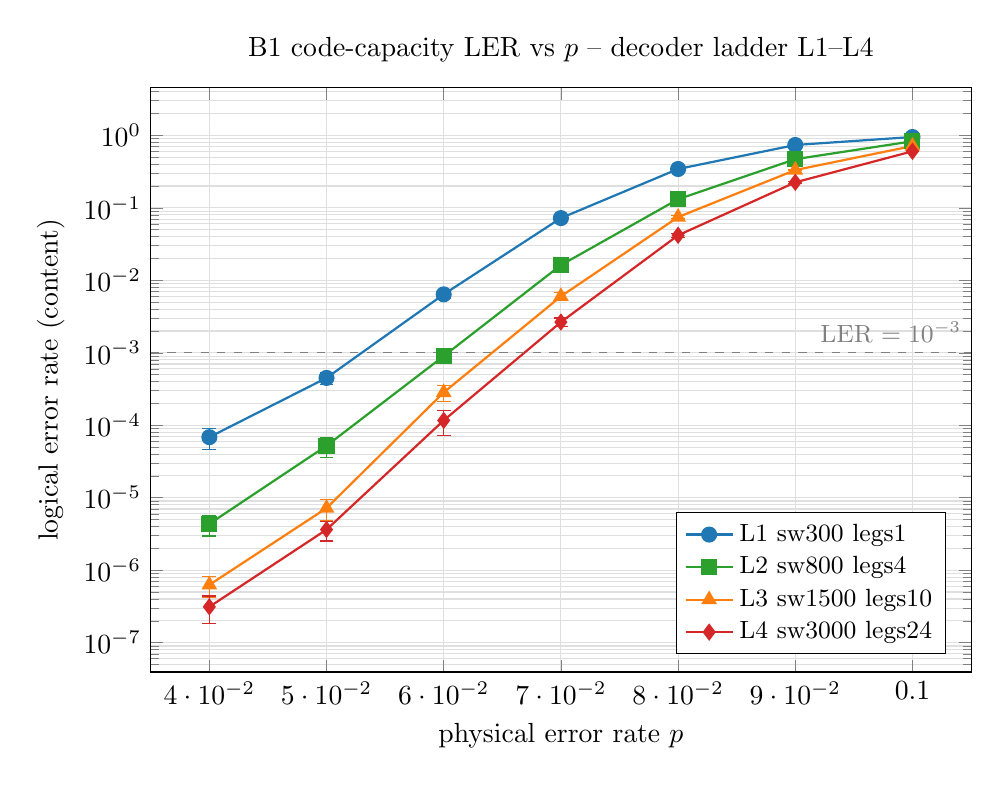
\begin{tikzpicture}
\begin{semilogyaxis}[
    width=12cm, height=9cm,
    xlabel={physical error rate $p$},
    ylabel={logical error rate (content)},
    title={B1 code-capacity LER vs $p$ -- decoder ladder L1--L4},
    xmin=0.035, xmax=0.105,
    xtick={0.04,0.05,0.06,0.07,0.08,0.09,0.1},
    grid=both, grid style={gray!25},
    legend pos=south east, legend cell align={left},
    legend style={font=\small},
    every axis plot/.append style={thick, mark options={solid}},
]
\addplot[color={rgb,255:red,31;green,119;blue,180}, mark=*, mark size=2.5pt,
    error bars/.cd, y dir=both, y explicit]
  coordinates {
    (0.04, 6.8490e-05) +- (0, 2.2000e-05)
    (0.05, 4.5000e-04) +- (0, 8.6603e-05)
    (0.06, 6.4000e-03) +- (0, 8.0000e-04)
    (0.07, 7.2200e-02) +- (0, 3.8000e-03)
    (0.08, 3.4340e-01) +- (0, 8.2873e-03)
    (0.09, 7.3660e-01) +- (0, 1.2138e-02)
    (0.1, 9.4880e-01) +- (0, 1.3775e-02)
  };
\addlegendentry{L1  sw300  legs1}
\addplot[color={rgb,255:red,44;green,160;blue,44}, mark=square*, mark size=2.5pt,
    error bars/.cd, y dir=both, y explicit]
  coordinates {
    (0.04, 4.3590e-06) +- (0, 1.4000e-06)
    (0.05, 5.2080e-05) +- (0, 1.6000e-05)
    (0.06, 9.0000e-04) +- (0, 1.5000e-04)
    (0.07, 1.6200e-02) +- (0, 1.8000e-03)
    (0.08, 1.3140e-01) +- (0, 5.1264e-03)
    (0.09, 4.6940e-01) +- (0, 9.6892e-03)
    (0.1, 8.2840e-01) +- (0, 1.2872e-02)
  };
\addlegendentry{L2  sw800  legs4}
\addplot[color={rgb,255:red,255;green,127;blue,14}, mark=triangle*, mark size=2.5pt,
    error bars/.cd, y dir=both, y explicit]
  coordinates {
    (0.04, 6.2740e-07) +- (0, 2.0000e-07)
    (0.05, 7.1840e-06) +- (0, 2.3000e-06)
    (0.06, 2.8333e-04) +- (0, 6.8718e-05)
    (0.07, 6.0000e-03) +- (0, 7.7460e-04)
    (0.08, 7.4600e-02) +- (0, 3.8626e-03)
    (0.09, 3.3200e-01) +- (0, 8.1486e-03)
    (0.1, 7.1240e-01) +- (0, 1.1936e-02)
  };
\addlegendentry{L3  sw1500 legs10}
\addplot[color={rgb,255:red,214;green,39;blue,40}, mark=diamond*, mark size=2.5pt,
    error bars/.cd, y dir=both, y explicit]
  coordinates {
    (0.04, 3.1247e-07) +- (0, 1.2756e-07)
    (0.05, 3.6310e-06) +- (0, 1.1000e-06)
    (0.06, 1.1667e-04) +- (0, 4.4096e-05)
    (0.07, 2.6500e-03) +- (0, 3.6401e-04)
    (0.08, 4.1800e-02) +- (0, 2.8914e-03)
    (0.09, 2.2480e-01) +- (0, 6.7052e-03)
    (0.1, 6.0280e-01) +- (0, 1.0980e-02)
  };
\addlegendentry{L4  sw3000 legs24}
\draw[dashed, gray] (axis cs:0.035,1e-3) -- (axis cs:0.105,1e-3);
\node[gray, font=\small, anchor=south east] at (axis cs:0.105,1e-3)
    {LER $=10^{-3}$};
\end{semilogyaxis}
\end{tikzpicture}

%
% Or compile this file on its own with:
%     \documentclass{standalone}
%     \usepackage{pgfplots}\pgfplotsset{compat=1.18}
%     \begin{document}% B1 code-capacity content-LER vs p -- decoder ladder L1-L4.
% Auto-generated by plot_ladder_ler.py -- do not edit by hand.
%
% In your document preamble:
%     \usepackage{pgfplots}
%     \pgfplotsset{compat=1.18}
% then in the body:
%     \input{b1_ladder_ler_vs_p.tex}
%
% Or compile this file on its own with:
%     \documentclass{standalone}
%     \usepackage{pgfplots}\pgfplotsset{compat=1.18}
%     \begin{document}\input{b1_ladder_ler_vs_p.tex}\end{document}
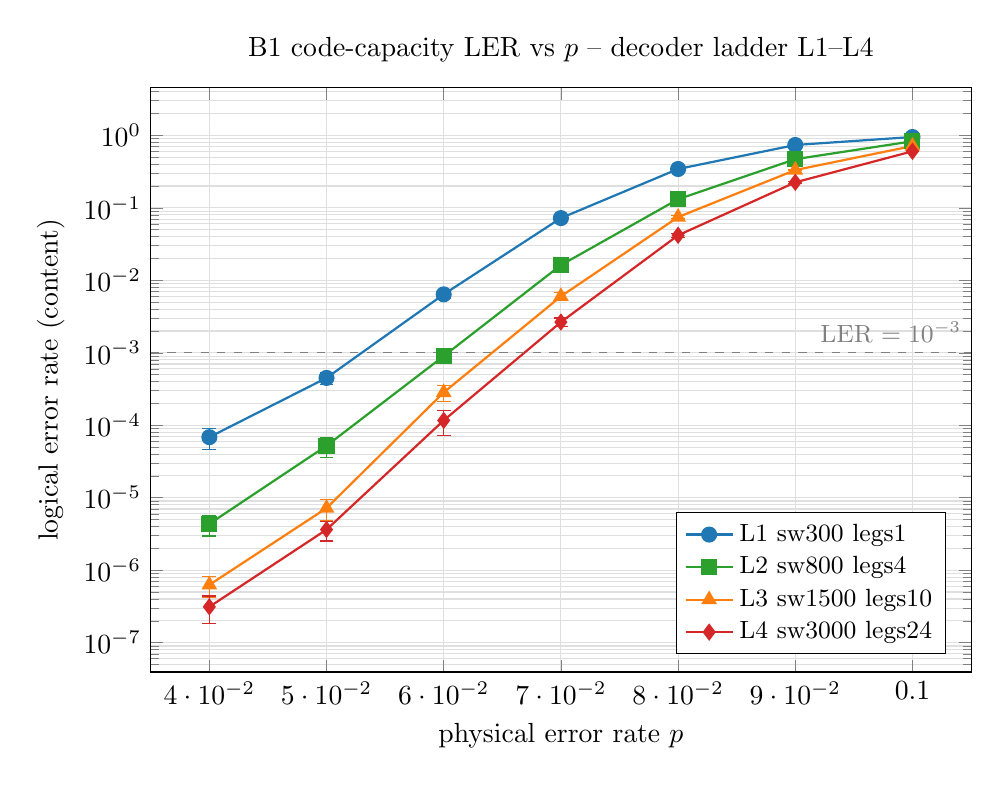
\begin{tikzpicture}
\begin{semilogyaxis}[
    width=12cm, height=9cm,
    xlabel={physical error rate $p$},
    ylabel={logical error rate (content)},
    title={B1 code-capacity LER vs $p$ -- decoder ladder L1--L4},
    xmin=0.035, xmax=0.105,
    xtick={0.04,0.05,0.06,0.07,0.08,0.09,0.1},
    grid=both, grid style={gray!25},
    legend pos=south east, legend cell align={left},
    legend style={font=\small},
    every axis plot/.append style={thick, mark options={solid}},
]
\addplot[color={rgb,255:red,31;green,119;blue,180}, mark=*, mark size=2.5pt,
    error bars/.cd, y dir=both, y explicit]
  coordinates {
    (0.04, 6.8490e-05) +- (0, 2.2000e-05)
    (0.05, 4.5000e-04) +- (0, 8.6603e-05)
    (0.06, 6.4000e-03) +- (0, 8.0000e-04)
    (0.07, 7.2200e-02) +- (0, 3.8000e-03)
    (0.08, 3.4340e-01) +- (0, 8.2873e-03)
    (0.09, 7.3660e-01) +- (0, 1.2138e-02)
    (0.1, 9.4880e-01) +- (0, 1.3775e-02)
  };
\addlegendentry{L1  sw300  legs1}
\addplot[color={rgb,255:red,44;green,160;blue,44}, mark=square*, mark size=2.5pt,
    error bars/.cd, y dir=both, y explicit]
  coordinates {
    (0.04, 4.3590e-06) +- (0, 1.4000e-06)
    (0.05, 5.2080e-05) +- (0, 1.6000e-05)
    (0.06, 9.0000e-04) +- (0, 1.5000e-04)
    (0.07, 1.6200e-02) +- (0, 1.8000e-03)
    (0.08, 1.3140e-01) +- (0, 5.1264e-03)
    (0.09, 4.6940e-01) +- (0, 9.6892e-03)
    (0.1, 8.2840e-01) +- (0, 1.2872e-02)
  };
\addlegendentry{L2  sw800  legs4}
\addplot[color={rgb,255:red,255;green,127;blue,14}, mark=triangle*, mark size=2.5pt,
    error bars/.cd, y dir=both, y explicit]
  coordinates {
    (0.04, 6.2740e-07) +- (0, 2.0000e-07)
    (0.05, 7.1840e-06) +- (0, 2.3000e-06)
    (0.06, 2.8333e-04) +- (0, 6.8718e-05)
    (0.07, 6.0000e-03) +- (0, 7.7460e-04)
    (0.08, 7.4600e-02) +- (0, 3.8626e-03)
    (0.09, 3.3200e-01) +- (0, 8.1486e-03)
    (0.1, 7.1240e-01) +- (0, 1.1936e-02)
  };
\addlegendentry{L3  sw1500 legs10}
\addplot[color={rgb,255:red,214;green,39;blue,40}, mark=diamond*, mark size=2.5pt,
    error bars/.cd, y dir=both, y explicit]
  coordinates {
    (0.04, 3.1247e-07) +- (0, 1.2756e-07)
    (0.05, 3.6310e-06) +- (0, 1.1000e-06)
    (0.06, 1.1667e-04) +- (0, 4.4096e-05)
    (0.07, 2.6500e-03) +- (0, 3.6401e-04)
    (0.08, 4.1800e-02) +- (0, 2.8914e-03)
    (0.09, 2.2480e-01) +- (0, 6.7052e-03)
    (0.1, 6.0280e-01) +- (0, 1.0980e-02)
  };
\addlegendentry{L4  sw3000 legs24}
\draw[dashed, gray] (axis cs:0.035,1e-3) -- (axis cs:0.105,1e-3);
\node[gray, font=\small, anchor=south east] at (axis cs:0.105,1e-3)
    {LER $=10^{-3}$};
\end{semilogyaxis}
\end{tikzpicture}
\end{document}
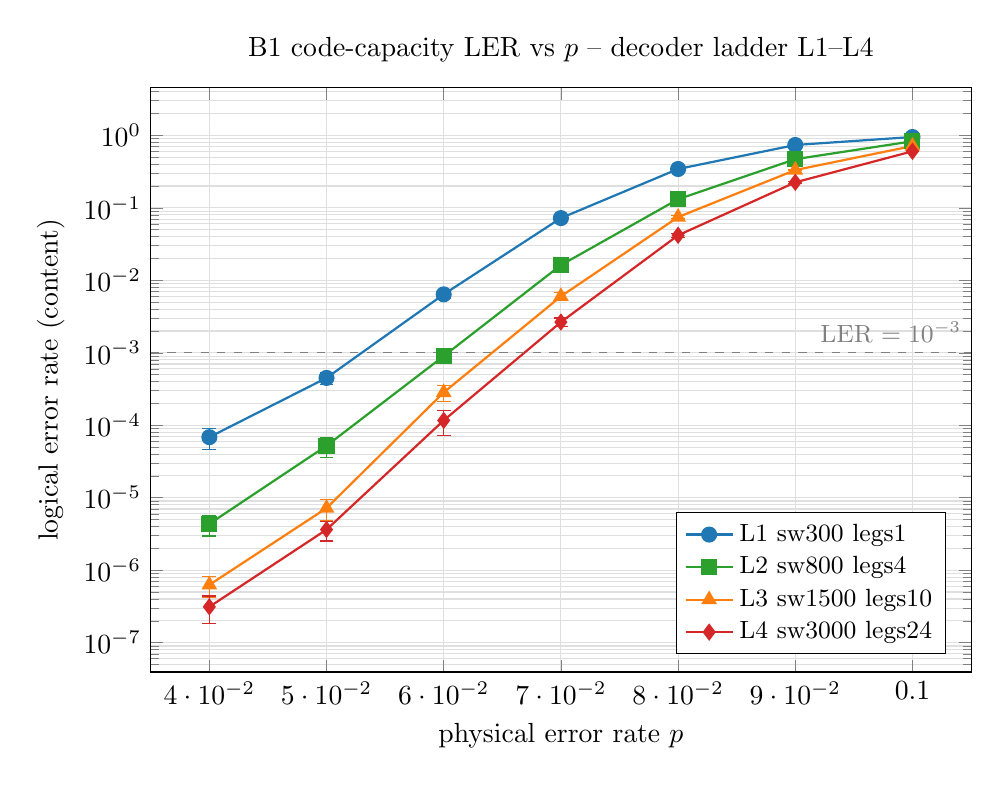
\begin{tikzpicture}
\begin{semilogyaxis}[
    width=12cm, height=9cm,
    xlabel={physical error rate $p$},
    ylabel={logical error rate (content)},
    title={B1 code-capacity LER vs $p$ -- decoder ladder L1--L4},
    xmin=0.035, xmax=0.105,
    xtick={0.04,0.05,0.06,0.07,0.08,0.09,0.1},
    grid=both, grid style={gray!25},
    legend pos=south east, legend cell align={left},
    legend style={font=\small},
    every axis plot/.append style={thick, mark options={solid}},
]
\addplot[color={rgb,255:red,31;green,119;blue,180}, mark=*, mark size=2.5pt,
    error bars/.cd, y dir=both, y explicit]
  coordinates {
    (0.04, 6.8490e-05) +- (0, 2.2000e-05)
    (0.05, 4.5000e-04) +- (0, 8.6603e-05)
    (0.06, 6.4000e-03) +- (0, 8.0000e-04)
    (0.07, 7.2200e-02) +- (0, 3.8000e-03)
    (0.08, 3.4340e-01) +- (0, 8.2873e-03)
    (0.09, 7.3660e-01) +- (0, 1.2138e-02)
    (0.1, 9.4880e-01) +- (0, 1.3775e-02)
  };
\addlegendentry{L1  sw300  legs1}
\addplot[color={rgb,255:red,44;green,160;blue,44}, mark=square*, mark size=2.5pt,
    error bars/.cd, y dir=both, y explicit]
  coordinates {
    (0.04, 4.3590e-06) +- (0, 1.4000e-06)
    (0.05, 5.2080e-05) +- (0, 1.6000e-05)
    (0.06, 9.0000e-04) +- (0, 1.5000e-04)
    (0.07, 1.6200e-02) +- (0, 1.8000e-03)
    (0.08, 1.3140e-01) +- (0, 5.1264e-03)
    (0.09, 4.6940e-01) +- (0, 9.6892e-03)
    (0.1, 8.2840e-01) +- (0, 1.2872e-02)
  };
\addlegendentry{L2  sw800  legs4}
\addplot[color={rgb,255:red,255;green,127;blue,14}, mark=triangle*, mark size=2.5pt,
    error bars/.cd, y dir=both, y explicit]
  coordinates {
    (0.04, 6.2740e-07) +- (0, 2.0000e-07)
    (0.05, 7.1840e-06) +- (0, 2.3000e-06)
    (0.06, 2.8333e-04) +- (0, 6.8718e-05)
    (0.07, 6.0000e-03) +- (0, 7.7460e-04)
    (0.08, 7.4600e-02) +- (0, 3.8626e-03)
    (0.09, 3.3200e-01) +- (0, 8.1486e-03)
    (0.1, 7.1240e-01) +- (0, 1.1936e-02)
  };
\addlegendentry{L3  sw1500 legs10}
\addplot[color={rgb,255:red,214;green,39;blue,40}, mark=diamond*, mark size=2.5pt,
    error bars/.cd, y dir=both, y explicit]
  coordinates {
    (0.04, 3.1247e-07) +- (0, 1.2756e-07)
    (0.05, 3.6310e-06) +- (0, 1.1000e-06)
    (0.06, 1.1667e-04) +- (0, 4.4096e-05)
    (0.07, 2.6500e-03) +- (0, 3.6401e-04)
    (0.08, 4.1800e-02) +- (0, 2.8914e-03)
    (0.09, 2.2480e-01) +- (0, 6.7052e-03)
    (0.1, 6.0280e-01) +- (0, 1.0980e-02)
  };
\addlegendentry{L4  sw3000 legs24}
\draw[dashed, gray] (axis cs:0.035,1e-3) -- (axis cs:0.105,1e-3);
\node[gray, font=\small, anchor=south east] at (axis cs:0.105,1e-3)
    {LER $=10^{-3}$};
\end{semilogyaxis}
\end{tikzpicture}

%
% Or compile this file on its own with:
%     \documentclass{standalone}
%     \usepackage{pgfplots}\pgfplotsset{compat=1.18}
%     \begin{document}% B1 code-capacity content-LER vs p -- decoder ladder L1-L4.
% Auto-generated by plot_ladder_ler.py -- do not edit by hand.
%
% In your document preamble:
%     \usepackage{pgfplots}
%     \pgfplotsset{compat=1.18}
% then in the body:
%     % B1 code-capacity content-LER vs p -- decoder ladder L1-L4.
% Auto-generated by plot_ladder_ler.py -- do not edit by hand.
%
% In your document preamble:
%     \usepackage{pgfplots}
%     \pgfplotsset{compat=1.18}
% then in the body:
%     \input{b1_ladder_ler_vs_p.tex}
%
% Or compile this file on its own with:
%     \documentclass{standalone}
%     \usepackage{pgfplots}\pgfplotsset{compat=1.18}
%     \begin{document}\input{b1_ladder_ler_vs_p.tex}\end{document}
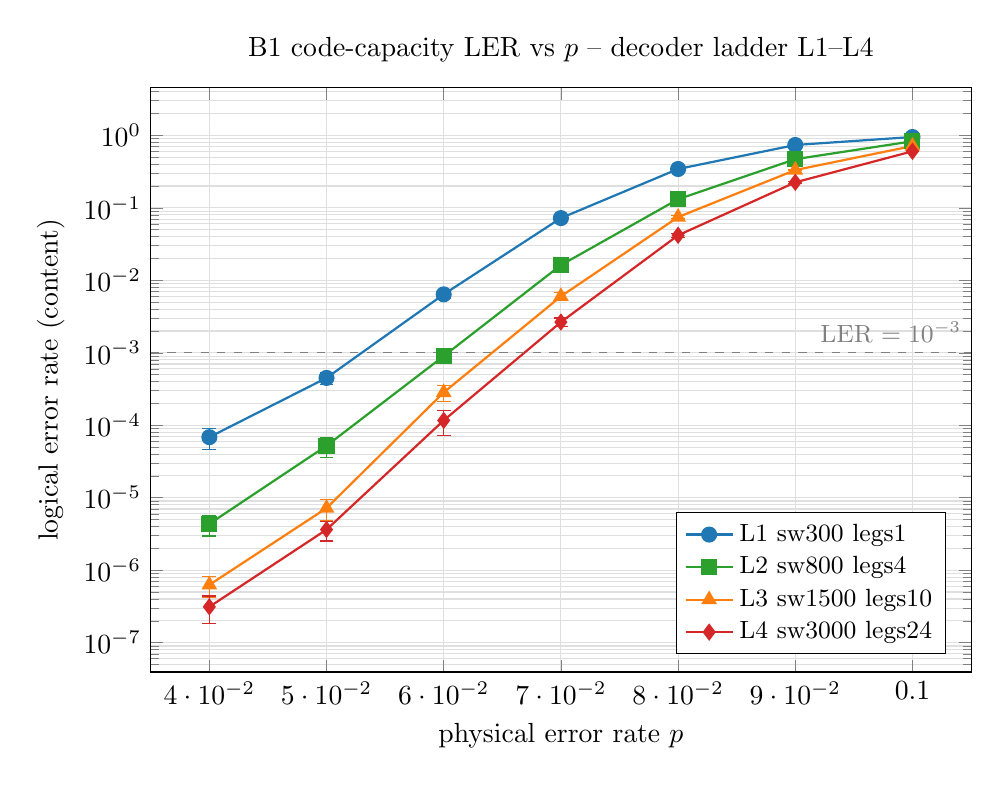
\begin{tikzpicture}
\begin{semilogyaxis}[
    width=12cm, height=9cm,
    xlabel={physical error rate $p$},
    ylabel={logical error rate (content)},
    title={B1 code-capacity LER vs $p$ -- decoder ladder L1--L4},
    xmin=0.035, xmax=0.105,
    xtick={0.04,0.05,0.06,0.07,0.08,0.09,0.1},
    grid=both, grid style={gray!25},
    legend pos=south east, legend cell align={left},
    legend style={font=\small},
    every axis plot/.append style={thick, mark options={solid}},
]
\addplot[color={rgb,255:red,31;green,119;blue,180}, mark=*, mark size=2.5pt,
    error bars/.cd, y dir=both, y explicit]
  coordinates {
    (0.04, 6.8490e-05) +- (0, 2.2000e-05)
    (0.05, 4.5000e-04) +- (0, 8.6603e-05)
    (0.06, 6.4000e-03) +- (0, 8.0000e-04)
    (0.07, 7.2200e-02) +- (0, 3.8000e-03)
    (0.08, 3.4340e-01) +- (0, 8.2873e-03)
    (0.09, 7.3660e-01) +- (0, 1.2138e-02)
    (0.1, 9.4880e-01) +- (0, 1.3775e-02)
  };
\addlegendentry{L1  sw300  legs1}
\addplot[color={rgb,255:red,44;green,160;blue,44}, mark=square*, mark size=2.5pt,
    error bars/.cd, y dir=both, y explicit]
  coordinates {
    (0.04, 4.3590e-06) +- (0, 1.4000e-06)
    (0.05, 5.2080e-05) +- (0, 1.6000e-05)
    (0.06, 9.0000e-04) +- (0, 1.5000e-04)
    (0.07, 1.6200e-02) +- (0, 1.8000e-03)
    (0.08, 1.3140e-01) +- (0, 5.1264e-03)
    (0.09, 4.6940e-01) +- (0, 9.6892e-03)
    (0.1, 8.2840e-01) +- (0, 1.2872e-02)
  };
\addlegendentry{L2  sw800  legs4}
\addplot[color={rgb,255:red,255;green,127;blue,14}, mark=triangle*, mark size=2.5pt,
    error bars/.cd, y dir=both, y explicit]
  coordinates {
    (0.04, 6.2740e-07) +- (0, 2.0000e-07)
    (0.05, 7.1840e-06) +- (0, 2.3000e-06)
    (0.06, 2.8333e-04) +- (0, 6.8718e-05)
    (0.07, 6.0000e-03) +- (0, 7.7460e-04)
    (0.08, 7.4600e-02) +- (0, 3.8626e-03)
    (0.09, 3.3200e-01) +- (0, 8.1486e-03)
    (0.1, 7.1240e-01) +- (0, 1.1936e-02)
  };
\addlegendentry{L3  sw1500 legs10}
\addplot[color={rgb,255:red,214;green,39;blue,40}, mark=diamond*, mark size=2.5pt,
    error bars/.cd, y dir=both, y explicit]
  coordinates {
    (0.04, 3.1247e-07) +- (0, 1.2756e-07)
    (0.05, 3.6310e-06) +- (0, 1.1000e-06)
    (0.06, 1.1667e-04) +- (0, 4.4096e-05)
    (0.07, 2.6500e-03) +- (0, 3.6401e-04)
    (0.08, 4.1800e-02) +- (0, 2.8914e-03)
    (0.09, 2.2480e-01) +- (0, 6.7052e-03)
    (0.1, 6.0280e-01) +- (0, 1.0980e-02)
  };
\addlegendentry{L4  sw3000 legs24}
\draw[dashed, gray] (axis cs:0.035,1e-3) -- (axis cs:0.105,1e-3);
\node[gray, font=\small, anchor=south east] at (axis cs:0.105,1e-3)
    {LER $=10^{-3}$};
\end{semilogyaxis}
\end{tikzpicture}

%
% Or compile this file on its own with:
%     \documentclass{standalone}
%     \usepackage{pgfplots}\pgfplotsset{compat=1.18}
%     \begin{document}% B1 code-capacity content-LER vs p -- decoder ladder L1-L4.
% Auto-generated by plot_ladder_ler.py -- do not edit by hand.
%
% In your document preamble:
%     \usepackage{pgfplots}
%     \pgfplotsset{compat=1.18}
% then in the body:
%     \input{b1_ladder_ler_vs_p.tex}
%
% Or compile this file on its own with:
%     \documentclass{standalone}
%     \usepackage{pgfplots}\pgfplotsset{compat=1.18}
%     \begin{document}\input{b1_ladder_ler_vs_p.tex}\end{document}
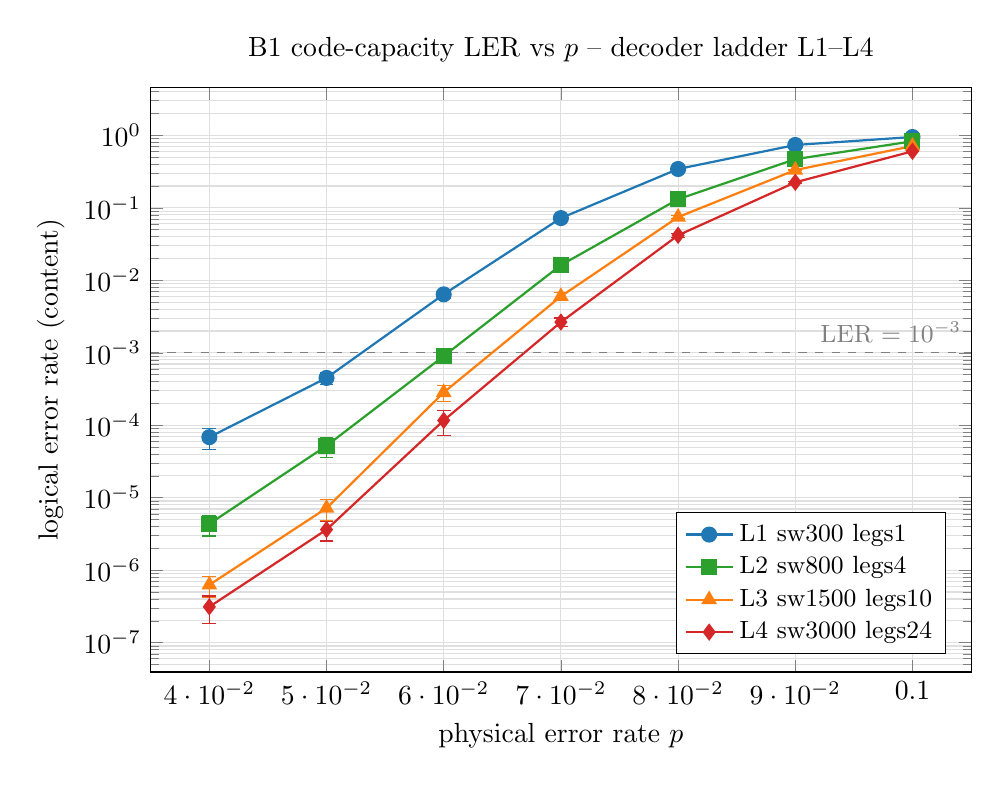
\begin{tikzpicture}
\begin{semilogyaxis}[
    width=12cm, height=9cm,
    xlabel={physical error rate $p$},
    ylabel={logical error rate (content)},
    title={B1 code-capacity LER vs $p$ -- decoder ladder L1--L4},
    xmin=0.035, xmax=0.105,
    xtick={0.04,0.05,0.06,0.07,0.08,0.09,0.1},
    grid=both, grid style={gray!25},
    legend pos=south east, legend cell align={left},
    legend style={font=\small},
    every axis plot/.append style={thick, mark options={solid}},
]
\addplot[color={rgb,255:red,31;green,119;blue,180}, mark=*, mark size=2.5pt,
    error bars/.cd, y dir=both, y explicit]
  coordinates {
    (0.04, 6.8490e-05) +- (0, 2.2000e-05)
    (0.05, 4.5000e-04) +- (0, 8.6603e-05)
    (0.06, 6.4000e-03) +- (0, 8.0000e-04)
    (0.07, 7.2200e-02) +- (0, 3.8000e-03)
    (0.08, 3.4340e-01) +- (0, 8.2873e-03)
    (0.09, 7.3660e-01) +- (0, 1.2138e-02)
    (0.1, 9.4880e-01) +- (0, 1.3775e-02)
  };
\addlegendentry{L1  sw300  legs1}
\addplot[color={rgb,255:red,44;green,160;blue,44}, mark=square*, mark size=2.5pt,
    error bars/.cd, y dir=both, y explicit]
  coordinates {
    (0.04, 4.3590e-06) +- (0, 1.4000e-06)
    (0.05, 5.2080e-05) +- (0, 1.6000e-05)
    (0.06, 9.0000e-04) +- (0, 1.5000e-04)
    (0.07, 1.6200e-02) +- (0, 1.8000e-03)
    (0.08, 1.3140e-01) +- (0, 5.1264e-03)
    (0.09, 4.6940e-01) +- (0, 9.6892e-03)
    (0.1, 8.2840e-01) +- (0, 1.2872e-02)
  };
\addlegendentry{L2  sw800  legs4}
\addplot[color={rgb,255:red,255;green,127;blue,14}, mark=triangle*, mark size=2.5pt,
    error bars/.cd, y dir=both, y explicit]
  coordinates {
    (0.04, 6.2740e-07) +- (0, 2.0000e-07)
    (0.05, 7.1840e-06) +- (0, 2.3000e-06)
    (0.06, 2.8333e-04) +- (0, 6.8718e-05)
    (0.07, 6.0000e-03) +- (0, 7.7460e-04)
    (0.08, 7.4600e-02) +- (0, 3.8626e-03)
    (0.09, 3.3200e-01) +- (0, 8.1486e-03)
    (0.1, 7.1240e-01) +- (0, 1.1936e-02)
  };
\addlegendentry{L3  sw1500 legs10}
\addplot[color={rgb,255:red,214;green,39;blue,40}, mark=diamond*, mark size=2.5pt,
    error bars/.cd, y dir=both, y explicit]
  coordinates {
    (0.04, 3.1247e-07) +- (0, 1.2756e-07)
    (0.05, 3.6310e-06) +- (0, 1.1000e-06)
    (0.06, 1.1667e-04) +- (0, 4.4096e-05)
    (0.07, 2.6500e-03) +- (0, 3.6401e-04)
    (0.08, 4.1800e-02) +- (0, 2.8914e-03)
    (0.09, 2.2480e-01) +- (0, 6.7052e-03)
    (0.1, 6.0280e-01) +- (0, 1.0980e-02)
  };
\addlegendentry{L4  sw3000 legs24}
\draw[dashed, gray] (axis cs:0.035,1e-3) -- (axis cs:0.105,1e-3);
\node[gray, font=\small, anchor=south east] at (axis cs:0.105,1e-3)
    {LER $=10^{-3}$};
\end{semilogyaxis}
\end{tikzpicture}
\end{document}
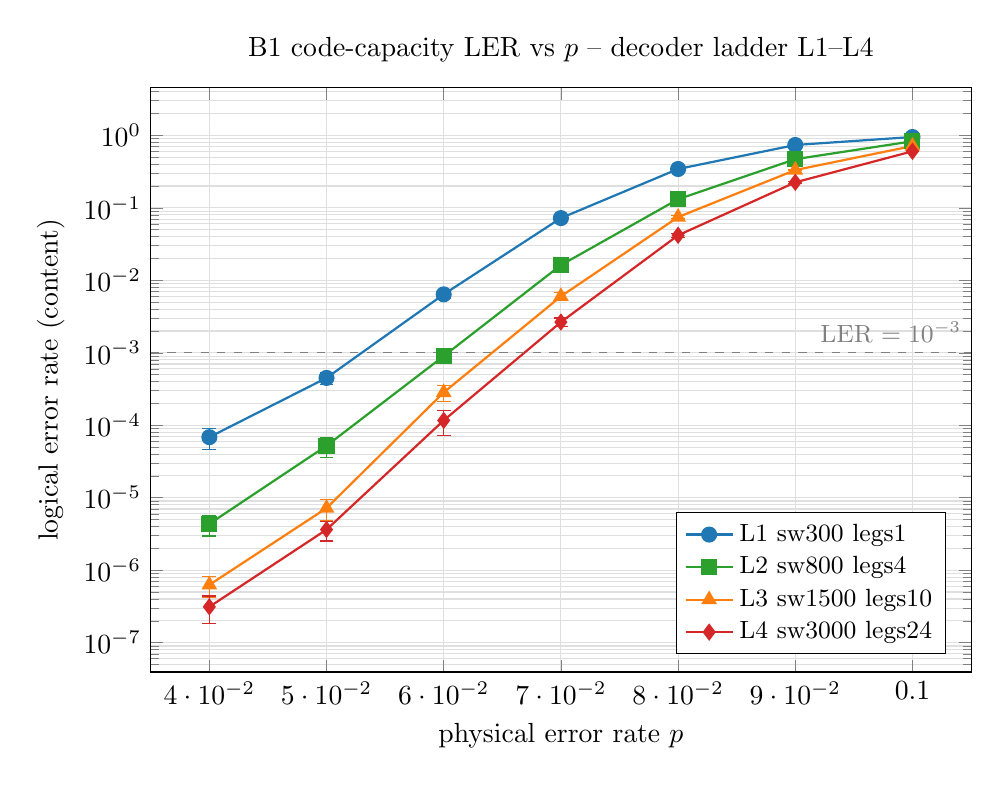
\begin{tikzpicture}
\begin{semilogyaxis}[
    width=12cm, height=9cm,
    xlabel={physical error rate $p$},
    ylabel={logical error rate (content)},
    title={B1 code-capacity LER vs $p$ -- decoder ladder L1--L4},
    xmin=0.035, xmax=0.105,
    xtick={0.04,0.05,0.06,0.07,0.08,0.09,0.1},
    grid=both, grid style={gray!25},
    legend pos=south east, legend cell align={left},
    legend style={font=\small},
    every axis plot/.append style={thick, mark options={solid}},
]
\addplot[color={rgb,255:red,31;green,119;blue,180}, mark=*, mark size=2.5pt,
    error bars/.cd, y dir=both, y explicit]
  coordinates {
    (0.04, 6.8490e-05) +- (0, 2.2000e-05)
    (0.05, 4.5000e-04) +- (0, 8.6603e-05)
    (0.06, 6.4000e-03) +- (0, 8.0000e-04)
    (0.07, 7.2200e-02) +- (0, 3.8000e-03)
    (0.08, 3.4340e-01) +- (0, 8.2873e-03)
    (0.09, 7.3660e-01) +- (0, 1.2138e-02)
    (0.1, 9.4880e-01) +- (0, 1.3775e-02)
  };
\addlegendentry{L1  sw300  legs1}
\addplot[color={rgb,255:red,44;green,160;blue,44}, mark=square*, mark size=2.5pt,
    error bars/.cd, y dir=both, y explicit]
  coordinates {
    (0.04, 4.3590e-06) +- (0, 1.4000e-06)
    (0.05, 5.2080e-05) +- (0, 1.6000e-05)
    (0.06, 9.0000e-04) +- (0, 1.5000e-04)
    (0.07, 1.6200e-02) +- (0, 1.8000e-03)
    (0.08, 1.3140e-01) +- (0, 5.1264e-03)
    (0.09, 4.6940e-01) +- (0, 9.6892e-03)
    (0.1, 8.2840e-01) +- (0, 1.2872e-02)
  };
\addlegendentry{L2  sw800  legs4}
\addplot[color={rgb,255:red,255;green,127;blue,14}, mark=triangle*, mark size=2.5pt,
    error bars/.cd, y dir=both, y explicit]
  coordinates {
    (0.04, 6.2740e-07) +- (0, 2.0000e-07)
    (0.05, 7.1840e-06) +- (0, 2.3000e-06)
    (0.06, 2.8333e-04) +- (0, 6.8718e-05)
    (0.07, 6.0000e-03) +- (0, 7.7460e-04)
    (0.08, 7.4600e-02) +- (0, 3.8626e-03)
    (0.09, 3.3200e-01) +- (0, 8.1486e-03)
    (0.1, 7.1240e-01) +- (0, 1.1936e-02)
  };
\addlegendentry{L3  sw1500 legs10}
\addplot[color={rgb,255:red,214;green,39;blue,40}, mark=diamond*, mark size=2.5pt,
    error bars/.cd, y dir=both, y explicit]
  coordinates {
    (0.04, 3.1247e-07) +- (0, 1.2756e-07)
    (0.05, 3.6310e-06) +- (0, 1.1000e-06)
    (0.06, 1.1667e-04) +- (0, 4.4096e-05)
    (0.07, 2.6500e-03) +- (0, 3.6401e-04)
    (0.08, 4.1800e-02) +- (0, 2.8914e-03)
    (0.09, 2.2480e-01) +- (0, 6.7052e-03)
    (0.1, 6.0280e-01) +- (0, 1.0980e-02)
  };
\addlegendentry{L4  sw3000 legs24}
\draw[dashed, gray] (axis cs:0.035,1e-3) -- (axis cs:0.105,1e-3);
\node[gray, font=\small, anchor=south east] at (axis cs:0.105,1e-3)
    {LER $=10^{-3}$};
\end{semilogyaxis}
\end{tikzpicture}
\end{document}
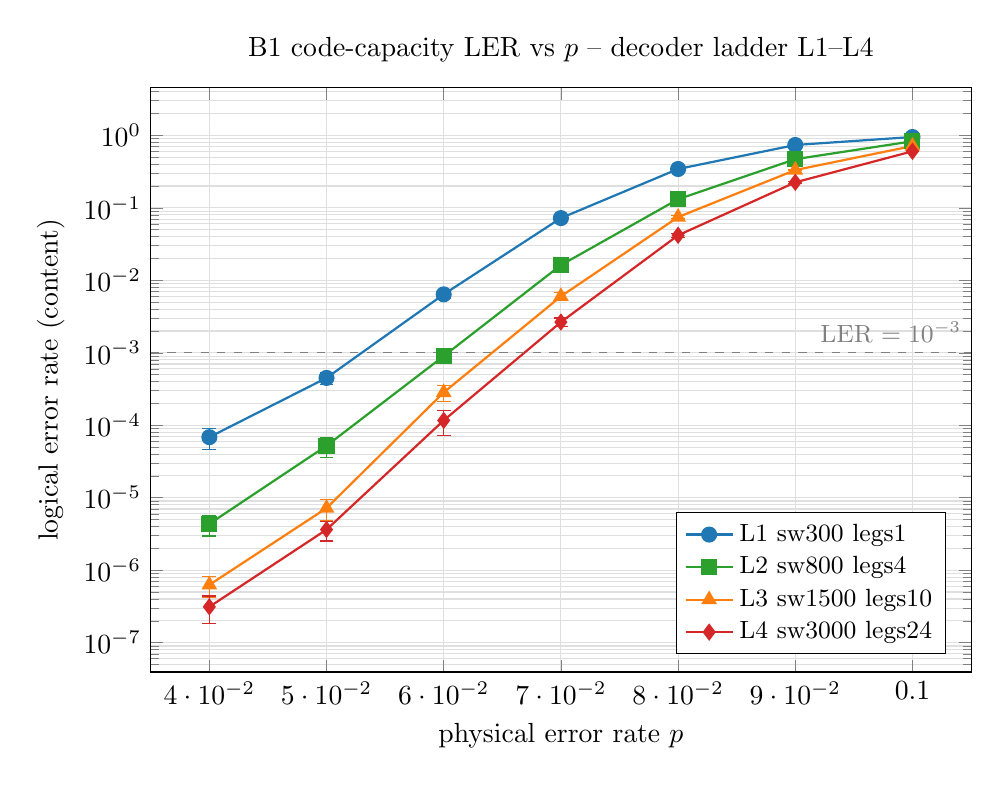
\begin{tikzpicture}
\begin{semilogyaxis}[
    width=12cm, height=9cm,
    xlabel={physical error rate $p$},
    ylabel={logical error rate (content)},
    title={B1 code-capacity LER vs $p$ -- decoder ladder L1--L4},
    xmin=0.035, xmax=0.105,
    xtick={0.04,0.05,0.06,0.07,0.08,0.09,0.1},
    grid=both, grid style={gray!25},
    legend pos=south east, legend cell align={left},
    legend style={font=\small},
    every axis plot/.append style={thick, mark options={solid}},
]
\addplot[color={rgb,255:red,31;green,119;blue,180}, mark=*, mark size=2.5pt,
    error bars/.cd, y dir=both, y explicit]
  coordinates {
    (0.04, 6.8490e-05) +- (0, 2.2000e-05)
    (0.05, 4.5000e-04) +- (0, 8.6603e-05)
    (0.06, 6.4000e-03) +- (0, 8.0000e-04)
    (0.07, 7.2200e-02) +- (0, 3.8000e-03)
    (0.08, 3.4340e-01) +- (0, 8.2873e-03)
    (0.09, 7.3660e-01) +- (0, 1.2138e-02)
    (0.1, 9.4880e-01) +- (0, 1.3775e-02)
  };
\addlegendentry{L1  sw300  legs1}
\addplot[color={rgb,255:red,44;green,160;blue,44}, mark=square*, mark size=2.5pt,
    error bars/.cd, y dir=both, y explicit]
  coordinates {
    (0.04, 4.3590e-06) +- (0, 1.4000e-06)
    (0.05, 5.2080e-05) +- (0, 1.6000e-05)
    (0.06, 9.0000e-04) +- (0, 1.5000e-04)
    (0.07, 1.6200e-02) +- (0, 1.8000e-03)
    (0.08, 1.3140e-01) +- (0, 5.1264e-03)
    (0.09, 4.6940e-01) +- (0, 9.6892e-03)
    (0.1, 8.2840e-01) +- (0, 1.2872e-02)
  };
\addlegendentry{L2  sw800  legs4}
\addplot[color={rgb,255:red,255;green,127;blue,14}, mark=triangle*, mark size=2.5pt,
    error bars/.cd, y dir=both, y explicit]
  coordinates {
    (0.04, 6.2740e-07) +- (0, 2.0000e-07)
    (0.05, 7.1840e-06) +- (0, 2.3000e-06)
    (0.06, 2.8333e-04) +- (0, 6.8718e-05)
    (0.07, 6.0000e-03) +- (0, 7.7460e-04)
    (0.08, 7.4600e-02) +- (0, 3.8626e-03)
    (0.09, 3.3200e-01) +- (0, 8.1486e-03)
    (0.1, 7.1240e-01) +- (0, 1.1936e-02)
  };
\addlegendentry{L3  sw1500 legs10}
\addplot[color={rgb,255:red,214;green,39;blue,40}, mark=diamond*, mark size=2.5pt,
    error bars/.cd, y dir=both, y explicit]
  coordinates {
    (0.04, 3.1247e-07) +- (0, 1.2756e-07)
    (0.05, 3.6310e-06) +- (0, 1.1000e-06)
    (0.06, 1.1667e-04) +- (0, 4.4096e-05)
    (0.07, 2.6500e-03) +- (0, 3.6401e-04)
    (0.08, 4.1800e-02) +- (0, 2.8914e-03)
    (0.09, 2.2480e-01) +- (0, 6.7052e-03)
    (0.1, 6.0280e-01) +- (0, 1.0980e-02)
  };
\addlegendentry{L4  sw3000 legs24}
\draw[dashed, gray] (axis cs:0.035,1e-3) -- (axis cs:0.105,1e-3);
\node[gray, font=\small, anchor=south east] at (axis cs:0.105,1e-3)
    {LER $=10^{-3}$};
\end{semilogyaxis}
\end{tikzpicture}

%
% Or compile this file on its own with:
%     \documentclass{standalone}
%     \usepackage{pgfplots}\pgfplotsset{compat=1.18}
%     \begin{document}% B1 code-capacity content-LER vs p -- decoder ladder L1-L4.
% Auto-generated by plot_ladder_ler.py -- do not edit by hand.
%
% In your document preamble:
%     \usepackage{pgfplots}
%     \pgfplotsset{compat=1.18}
% then in the body:
%     % B1 code-capacity content-LER vs p -- decoder ladder L1-L4.
% Auto-generated by plot_ladder_ler.py -- do not edit by hand.
%
% In your document preamble:
%     \usepackage{pgfplots}
%     \pgfplotsset{compat=1.18}
% then in the body:
%     % B1 code-capacity content-LER vs p -- decoder ladder L1-L4.
% Auto-generated by plot_ladder_ler.py -- do not edit by hand.
%
% In your document preamble:
%     \usepackage{pgfplots}
%     \pgfplotsset{compat=1.18}
% then in the body:
%     \input{b1_ladder_ler_vs_p.tex}
%
% Or compile this file on its own with:
%     \documentclass{standalone}
%     \usepackage{pgfplots}\pgfplotsset{compat=1.18}
%     \begin{document}\input{b1_ladder_ler_vs_p.tex}\end{document}
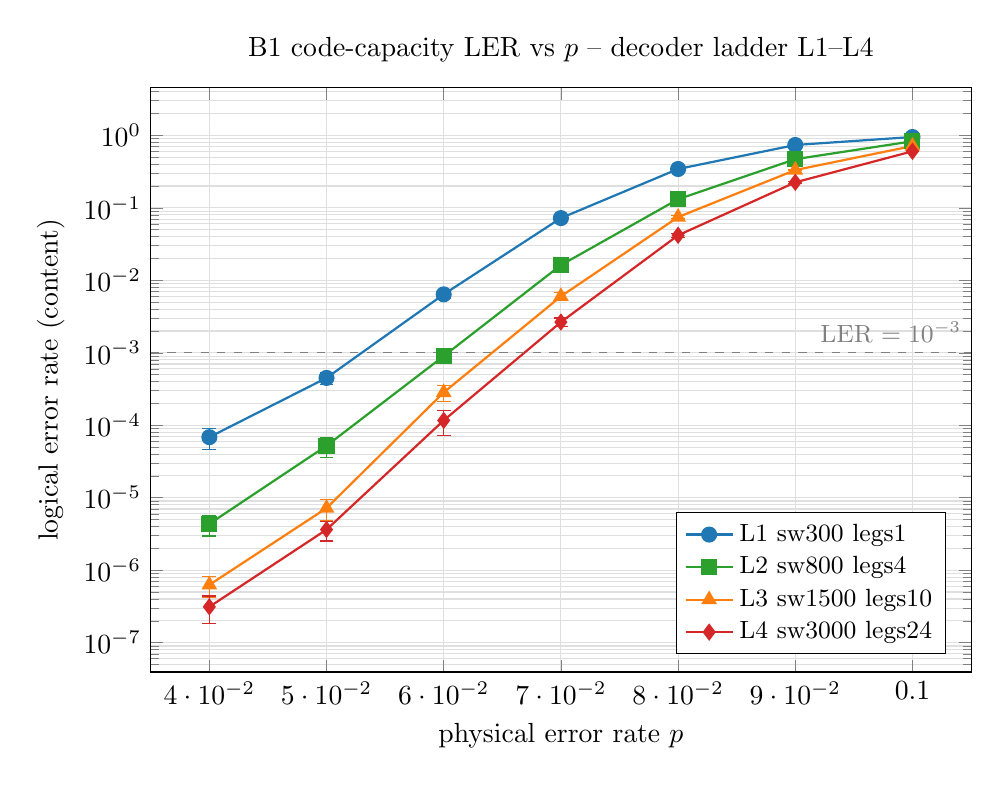
\begin{tikzpicture}
\begin{semilogyaxis}[
    width=12cm, height=9cm,
    xlabel={physical error rate $p$},
    ylabel={logical error rate (content)},
    title={B1 code-capacity LER vs $p$ -- decoder ladder L1--L4},
    xmin=0.035, xmax=0.105,
    xtick={0.04,0.05,0.06,0.07,0.08,0.09,0.1},
    grid=both, grid style={gray!25},
    legend pos=south east, legend cell align={left},
    legend style={font=\small},
    every axis plot/.append style={thick, mark options={solid}},
]
\addplot[color={rgb,255:red,31;green,119;blue,180}, mark=*, mark size=2.5pt,
    error bars/.cd, y dir=both, y explicit]
  coordinates {
    (0.04, 6.8490e-05) +- (0, 2.2000e-05)
    (0.05, 4.5000e-04) +- (0, 8.6603e-05)
    (0.06, 6.4000e-03) +- (0, 8.0000e-04)
    (0.07, 7.2200e-02) +- (0, 3.8000e-03)
    (0.08, 3.4340e-01) +- (0, 8.2873e-03)
    (0.09, 7.3660e-01) +- (0, 1.2138e-02)
    (0.1, 9.4880e-01) +- (0, 1.3775e-02)
  };
\addlegendentry{L1  sw300  legs1}
\addplot[color={rgb,255:red,44;green,160;blue,44}, mark=square*, mark size=2.5pt,
    error bars/.cd, y dir=both, y explicit]
  coordinates {
    (0.04, 4.3590e-06) +- (0, 1.4000e-06)
    (0.05, 5.2080e-05) +- (0, 1.6000e-05)
    (0.06, 9.0000e-04) +- (0, 1.5000e-04)
    (0.07, 1.6200e-02) +- (0, 1.8000e-03)
    (0.08, 1.3140e-01) +- (0, 5.1264e-03)
    (0.09, 4.6940e-01) +- (0, 9.6892e-03)
    (0.1, 8.2840e-01) +- (0, 1.2872e-02)
  };
\addlegendentry{L2  sw800  legs4}
\addplot[color={rgb,255:red,255;green,127;blue,14}, mark=triangle*, mark size=2.5pt,
    error bars/.cd, y dir=both, y explicit]
  coordinates {
    (0.04, 6.2740e-07) +- (0, 2.0000e-07)
    (0.05, 7.1840e-06) +- (0, 2.3000e-06)
    (0.06, 2.8333e-04) +- (0, 6.8718e-05)
    (0.07, 6.0000e-03) +- (0, 7.7460e-04)
    (0.08, 7.4600e-02) +- (0, 3.8626e-03)
    (0.09, 3.3200e-01) +- (0, 8.1486e-03)
    (0.1, 7.1240e-01) +- (0, 1.1936e-02)
  };
\addlegendentry{L3  sw1500 legs10}
\addplot[color={rgb,255:red,214;green,39;blue,40}, mark=diamond*, mark size=2.5pt,
    error bars/.cd, y dir=both, y explicit]
  coordinates {
    (0.04, 3.1247e-07) +- (0, 1.2756e-07)
    (0.05, 3.6310e-06) +- (0, 1.1000e-06)
    (0.06, 1.1667e-04) +- (0, 4.4096e-05)
    (0.07, 2.6500e-03) +- (0, 3.6401e-04)
    (0.08, 4.1800e-02) +- (0, 2.8914e-03)
    (0.09, 2.2480e-01) +- (0, 6.7052e-03)
    (0.1, 6.0280e-01) +- (0, 1.0980e-02)
  };
\addlegendentry{L4  sw3000 legs24}
\draw[dashed, gray] (axis cs:0.035,1e-3) -- (axis cs:0.105,1e-3);
\node[gray, font=\small, anchor=south east] at (axis cs:0.105,1e-3)
    {LER $=10^{-3}$};
\end{semilogyaxis}
\end{tikzpicture}

%
% Or compile this file on its own with:
%     \documentclass{standalone}
%     \usepackage{pgfplots}\pgfplotsset{compat=1.18}
%     \begin{document}% B1 code-capacity content-LER vs p -- decoder ladder L1-L4.
% Auto-generated by plot_ladder_ler.py -- do not edit by hand.
%
% In your document preamble:
%     \usepackage{pgfplots}
%     \pgfplotsset{compat=1.18}
% then in the body:
%     \input{b1_ladder_ler_vs_p.tex}
%
% Or compile this file on its own with:
%     \documentclass{standalone}
%     \usepackage{pgfplots}\pgfplotsset{compat=1.18}
%     \begin{document}\input{b1_ladder_ler_vs_p.tex}\end{document}
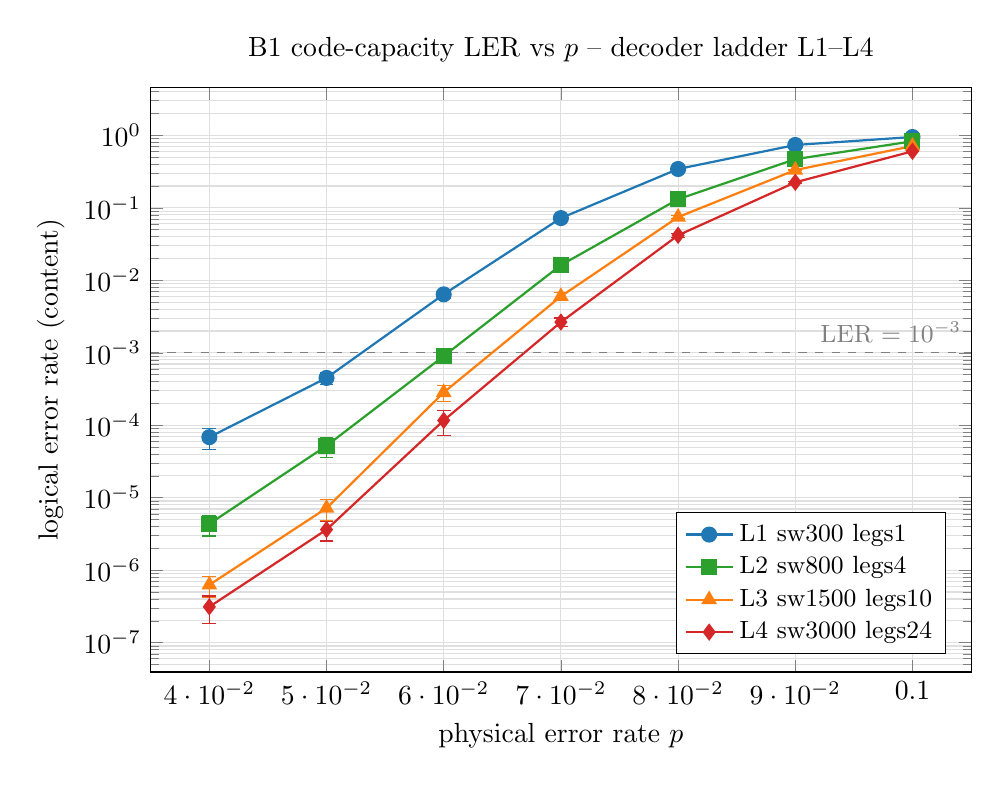
\begin{tikzpicture}
\begin{semilogyaxis}[
    width=12cm, height=9cm,
    xlabel={physical error rate $p$},
    ylabel={logical error rate (content)},
    title={B1 code-capacity LER vs $p$ -- decoder ladder L1--L4},
    xmin=0.035, xmax=0.105,
    xtick={0.04,0.05,0.06,0.07,0.08,0.09,0.1},
    grid=both, grid style={gray!25},
    legend pos=south east, legend cell align={left},
    legend style={font=\small},
    every axis plot/.append style={thick, mark options={solid}},
]
\addplot[color={rgb,255:red,31;green,119;blue,180}, mark=*, mark size=2.5pt,
    error bars/.cd, y dir=both, y explicit]
  coordinates {
    (0.04, 6.8490e-05) +- (0, 2.2000e-05)
    (0.05, 4.5000e-04) +- (0, 8.6603e-05)
    (0.06, 6.4000e-03) +- (0, 8.0000e-04)
    (0.07, 7.2200e-02) +- (0, 3.8000e-03)
    (0.08, 3.4340e-01) +- (0, 8.2873e-03)
    (0.09, 7.3660e-01) +- (0, 1.2138e-02)
    (0.1, 9.4880e-01) +- (0, 1.3775e-02)
  };
\addlegendentry{L1  sw300  legs1}
\addplot[color={rgb,255:red,44;green,160;blue,44}, mark=square*, mark size=2.5pt,
    error bars/.cd, y dir=both, y explicit]
  coordinates {
    (0.04, 4.3590e-06) +- (0, 1.4000e-06)
    (0.05, 5.2080e-05) +- (0, 1.6000e-05)
    (0.06, 9.0000e-04) +- (0, 1.5000e-04)
    (0.07, 1.6200e-02) +- (0, 1.8000e-03)
    (0.08, 1.3140e-01) +- (0, 5.1264e-03)
    (0.09, 4.6940e-01) +- (0, 9.6892e-03)
    (0.1, 8.2840e-01) +- (0, 1.2872e-02)
  };
\addlegendentry{L2  sw800  legs4}
\addplot[color={rgb,255:red,255;green,127;blue,14}, mark=triangle*, mark size=2.5pt,
    error bars/.cd, y dir=both, y explicit]
  coordinates {
    (0.04, 6.2740e-07) +- (0, 2.0000e-07)
    (0.05, 7.1840e-06) +- (0, 2.3000e-06)
    (0.06, 2.8333e-04) +- (0, 6.8718e-05)
    (0.07, 6.0000e-03) +- (0, 7.7460e-04)
    (0.08, 7.4600e-02) +- (0, 3.8626e-03)
    (0.09, 3.3200e-01) +- (0, 8.1486e-03)
    (0.1, 7.1240e-01) +- (0, 1.1936e-02)
  };
\addlegendentry{L3  sw1500 legs10}
\addplot[color={rgb,255:red,214;green,39;blue,40}, mark=diamond*, mark size=2.5pt,
    error bars/.cd, y dir=both, y explicit]
  coordinates {
    (0.04, 3.1247e-07) +- (0, 1.2756e-07)
    (0.05, 3.6310e-06) +- (0, 1.1000e-06)
    (0.06, 1.1667e-04) +- (0, 4.4096e-05)
    (0.07, 2.6500e-03) +- (0, 3.6401e-04)
    (0.08, 4.1800e-02) +- (0, 2.8914e-03)
    (0.09, 2.2480e-01) +- (0, 6.7052e-03)
    (0.1, 6.0280e-01) +- (0, 1.0980e-02)
  };
\addlegendentry{L4  sw3000 legs24}
\draw[dashed, gray] (axis cs:0.035,1e-3) -- (axis cs:0.105,1e-3);
\node[gray, font=\small, anchor=south east] at (axis cs:0.105,1e-3)
    {LER $=10^{-3}$};
\end{semilogyaxis}
\end{tikzpicture}
\end{document}
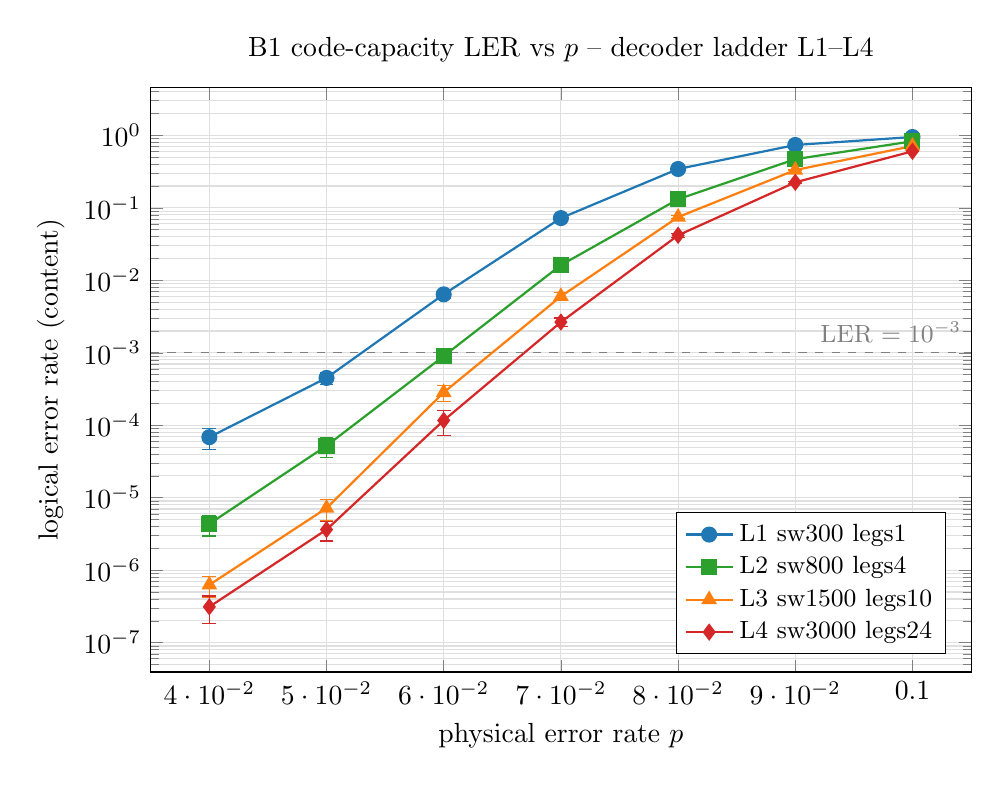
\begin{tikzpicture}
\begin{semilogyaxis}[
    width=12cm, height=9cm,
    xlabel={physical error rate $p$},
    ylabel={logical error rate (content)},
    title={B1 code-capacity LER vs $p$ -- decoder ladder L1--L4},
    xmin=0.035, xmax=0.105,
    xtick={0.04,0.05,0.06,0.07,0.08,0.09,0.1},
    grid=both, grid style={gray!25},
    legend pos=south east, legend cell align={left},
    legend style={font=\small},
    every axis plot/.append style={thick, mark options={solid}},
]
\addplot[color={rgb,255:red,31;green,119;blue,180}, mark=*, mark size=2.5pt,
    error bars/.cd, y dir=both, y explicit]
  coordinates {
    (0.04, 6.8490e-05) +- (0, 2.2000e-05)
    (0.05, 4.5000e-04) +- (0, 8.6603e-05)
    (0.06, 6.4000e-03) +- (0, 8.0000e-04)
    (0.07, 7.2200e-02) +- (0, 3.8000e-03)
    (0.08, 3.4340e-01) +- (0, 8.2873e-03)
    (0.09, 7.3660e-01) +- (0, 1.2138e-02)
    (0.1, 9.4880e-01) +- (0, 1.3775e-02)
  };
\addlegendentry{L1  sw300  legs1}
\addplot[color={rgb,255:red,44;green,160;blue,44}, mark=square*, mark size=2.5pt,
    error bars/.cd, y dir=both, y explicit]
  coordinates {
    (0.04, 4.3590e-06) +- (0, 1.4000e-06)
    (0.05, 5.2080e-05) +- (0, 1.6000e-05)
    (0.06, 9.0000e-04) +- (0, 1.5000e-04)
    (0.07, 1.6200e-02) +- (0, 1.8000e-03)
    (0.08, 1.3140e-01) +- (0, 5.1264e-03)
    (0.09, 4.6940e-01) +- (0, 9.6892e-03)
    (0.1, 8.2840e-01) +- (0, 1.2872e-02)
  };
\addlegendentry{L2  sw800  legs4}
\addplot[color={rgb,255:red,255;green,127;blue,14}, mark=triangle*, mark size=2.5pt,
    error bars/.cd, y dir=both, y explicit]
  coordinates {
    (0.04, 6.2740e-07) +- (0, 2.0000e-07)
    (0.05, 7.1840e-06) +- (0, 2.3000e-06)
    (0.06, 2.8333e-04) +- (0, 6.8718e-05)
    (0.07, 6.0000e-03) +- (0, 7.7460e-04)
    (0.08, 7.4600e-02) +- (0, 3.8626e-03)
    (0.09, 3.3200e-01) +- (0, 8.1486e-03)
    (0.1, 7.1240e-01) +- (0, 1.1936e-02)
  };
\addlegendentry{L3  sw1500 legs10}
\addplot[color={rgb,255:red,214;green,39;blue,40}, mark=diamond*, mark size=2.5pt,
    error bars/.cd, y dir=both, y explicit]
  coordinates {
    (0.04, 3.1247e-07) +- (0, 1.2756e-07)
    (0.05, 3.6310e-06) +- (0, 1.1000e-06)
    (0.06, 1.1667e-04) +- (0, 4.4096e-05)
    (0.07, 2.6500e-03) +- (0, 3.6401e-04)
    (0.08, 4.1800e-02) +- (0, 2.8914e-03)
    (0.09, 2.2480e-01) +- (0, 6.7052e-03)
    (0.1, 6.0280e-01) +- (0, 1.0980e-02)
  };
\addlegendentry{L4  sw3000 legs24}
\draw[dashed, gray] (axis cs:0.035,1e-3) -- (axis cs:0.105,1e-3);
\node[gray, font=\small, anchor=south east] at (axis cs:0.105,1e-3)
    {LER $=10^{-3}$};
\end{semilogyaxis}
\end{tikzpicture}

%
% Or compile this file on its own with:
%     \documentclass{standalone}
%     \usepackage{pgfplots}\pgfplotsset{compat=1.18}
%     \begin{document}% B1 code-capacity content-LER vs p -- decoder ladder L1-L4.
% Auto-generated by plot_ladder_ler.py -- do not edit by hand.
%
% In your document preamble:
%     \usepackage{pgfplots}
%     \pgfplotsset{compat=1.18}
% then in the body:
%     % B1 code-capacity content-LER vs p -- decoder ladder L1-L4.
% Auto-generated by plot_ladder_ler.py -- do not edit by hand.
%
% In your document preamble:
%     \usepackage{pgfplots}
%     \pgfplotsset{compat=1.18}
% then in the body:
%     \input{b1_ladder_ler_vs_p.tex}
%
% Or compile this file on its own with:
%     \documentclass{standalone}
%     \usepackage{pgfplots}\pgfplotsset{compat=1.18}
%     \begin{document}\input{b1_ladder_ler_vs_p.tex}\end{document}
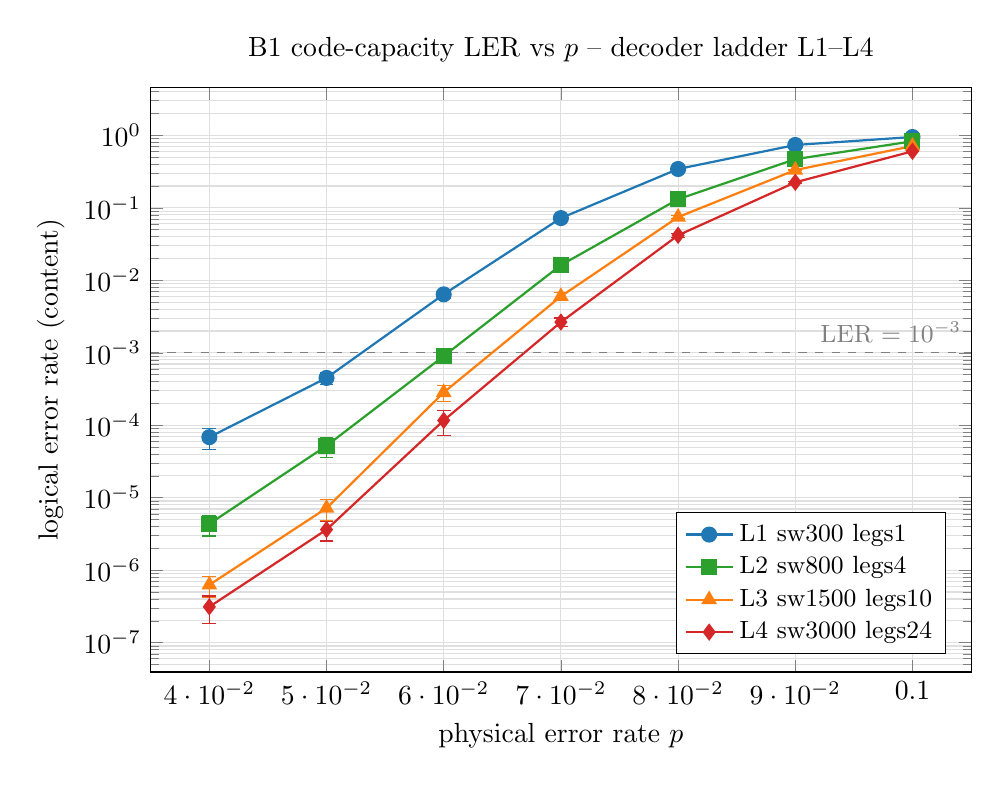
\begin{tikzpicture}
\begin{semilogyaxis}[
    width=12cm, height=9cm,
    xlabel={physical error rate $p$},
    ylabel={logical error rate (content)},
    title={B1 code-capacity LER vs $p$ -- decoder ladder L1--L4},
    xmin=0.035, xmax=0.105,
    xtick={0.04,0.05,0.06,0.07,0.08,0.09,0.1},
    grid=both, grid style={gray!25},
    legend pos=south east, legend cell align={left},
    legend style={font=\small},
    every axis plot/.append style={thick, mark options={solid}},
]
\addplot[color={rgb,255:red,31;green,119;blue,180}, mark=*, mark size=2.5pt,
    error bars/.cd, y dir=both, y explicit]
  coordinates {
    (0.04, 6.8490e-05) +- (0, 2.2000e-05)
    (0.05, 4.5000e-04) +- (0, 8.6603e-05)
    (0.06, 6.4000e-03) +- (0, 8.0000e-04)
    (0.07, 7.2200e-02) +- (0, 3.8000e-03)
    (0.08, 3.4340e-01) +- (0, 8.2873e-03)
    (0.09, 7.3660e-01) +- (0, 1.2138e-02)
    (0.1, 9.4880e-01) +- (0, 1.3775e-02)
  };
\addlegendentry{L1  sw300  legs1}
\addplot[color={rgb,255:red,44;green,160;blue,44}, mark=square*, mark size=2.5pt,
    error bars/.cd, y dir=both, y explicit]
  coordinates {
    (0.04, 4.3590e-06) +- (0, 1.4000e-06)
    (0.05, 5.2080e-05) +- (0, 1.6000e-05)
    (0.06, 9.0000e-04) +- (0, 1.5000e-04)
    (0.07, 1.6200e-02) +- (0, 1.8000e-03)
    (0.08, 1.3140e-01) +- (0, 5.1264e-03)
    (0.09, 4.6940e-01) +- (0, 9.6892e-03)
    (0.1, 8.2840e-01) +- (0, 1.2872e-02)
  };
\addlegendentry{L2  sw800  legs4}
\addplot[color={rgb,255:red,255;green,127;blue,14}, mark=triangle*, mark size=2.5pt,
    error bars/.cd, y dir=both, y explicit]
  coordinates {
    (0.04, 6.2740e-07) +- (0, 2.0000e-07)
    (0.05, 7.1840e-06) +- (0, 2.3000e-06)
    (0.06, 2.8333e-04) +- (0, 6.8718e-05)
    (0.07, 6.0000e-03) +- (0, 7.7460e-04)
    (0.08, 7.4600e-02) +- (0, 3.8626e-03)
    (0.09, 3.3200e-01) +- (0, 8.1486e-03)
    (0.1, 7.1240e-01) +- (0, 1.1936e-02)
  };
\addlegendentry{L3  sw1500 legs10}
\addplot[color={rgb,255:red,214;green,39;blue,40}, mark=diamond*, mark size=2.5pt,
    error bars/.cd, y dir=both, y explicit]
  coordinates {
    (0.04, 3.1247e-07) +- (0, 1.2756e-07)
    (0.05, 3.6310e-06) +- (0, 1.1000e-06)
    (0.06, 1.1667e-04) +- (0, 4.4096e-05)
    (0.07, 2.6500e-03) +- (0, 3.6401e-04)
    (0.08, 4.1800e-02) +- (0, 2.8914e-03)
    (0.09, 2.2480e-01) +- (0, 6.7052e-03)
    (0.1, 6.0280e-01) +- (0, 1.0980e-02)
  };
\addlegendentry{L4  sw3000 legs24}
\draw[dashed, gray] (axis cs:0.035,1e-3) -- (axis cs:0.105,1e-3);
\node[gray, font=\small, anchor=south east] at (axis cs:0.105,1e-3)
    {LER $=10^{-3}$};
\end{semilogyaxis}
\end{tikzpicture}

%
% Or compile this file on its own with:
%     \documentclass{standalone}
%     \usepackage{pgfplots}\pgfplotsset{compat=1.18}
%     \begin{document}% B1 code-capacity content-LER vs p -- decoder ladder L1-L4.
% Auto-generated by plot_ladder_ler.py -- do not edit by hand.
%
% In your document preamble:
%     \usepackage{pgfplots}
%     \pgfplotsset{compat=1.18}
% then in the body:
%     \input{b1_ladder_ler_vs_p.tex}
%
% Or compile this file on its own with:
%     \documentclass{standalone}
%     \usepackage{pgfplots}\pgfplotsset{compat=1.18}
%     \begin{document}\input{b1_ladder_ler_vs_p.tex}\end{document}
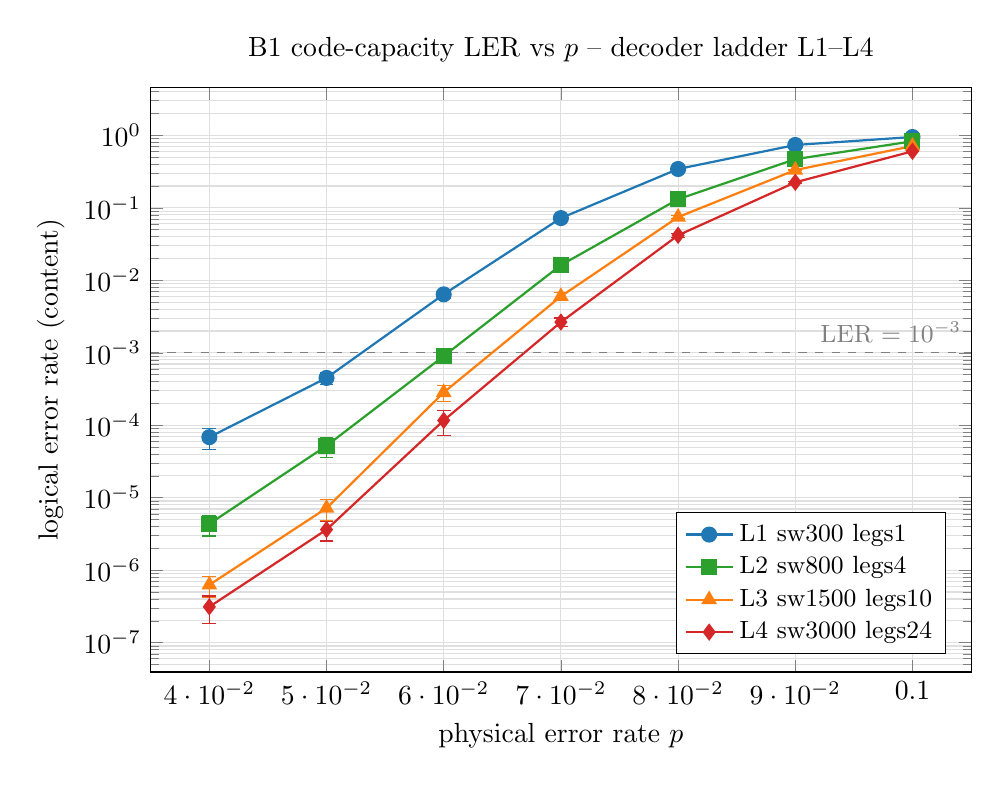
\begin{tikzpicture}
\begin{semilogyaxis}[
    width=12cm, height=9cm,
    xlabel={physical error rate $p$},
    ylabel={logical error rate (content)},
    title={B1 code-capacity LER vs $p$ -- decoder ladder L1--L4},
    xmin=0.035, xmax=0.105,
    xtick={0.04,0.05,0.06,0.07,0.08,0.09,0.1},
    grid=both, grid style={gray!25},
    legend pos=south east, legend cell align={left},
    legend style={font=\small},
    every axis plot/.append style={thick, mark options={solid}},
]
\addplot[color={rgb,255:red,31;green,119;blue,180}, mark=*, mark size=2.5pt,
    error bars/.cd, y dir=both, y explicit]
  coordinates {
    (0.04, 6.8490e-05) +- (0, 2.2000e-05)
    (0.05, 4.5000e-04) +- (0, 8.6603e-05)
    (0.06, 6.4000e-03) +- (0, 8.0000e-04)
    (0.07, 7.2200e-02) +- (0, 3.8000e-03)
    (0.08, 3.4340e-01) +- (0, 8.2873e-03)
    (0.09, 7.3660e-01) +- (0, 1.2138e-02)
    (0.1, 9.4880e-01) +- (0, 1.3775e-02)
  };
\addlegendentry{L1  sw300  legs1}
\addplot[color={rgb,255:red,44;green,160;blue,44}, mark=square*, mark size=2.5pt,
    error bars/.cd, y dir=both, y explicit]
  coordinates {
    (0.04, 4.3590e-06) +- (0, 1.4000e-06)
    (0.05, 5.2080e-05) +- (0, 1.6000e-05)
    (0.06, 9.0000e-04) +- (0, 1.5000e-04)
    (0.07, 1.6200e-02) +- (0, 1.8000e-03)
    (0.08, 1.3140e-01) +- (0, 5.1264e-03)
    (0.09, 4.6940e-01) +- (0, 9.6892e-03)
    (0.1, 8.2840e-01) +- (0, 1.2872e-02)
  };
\addlegendentry{L2  sw800  legs4}
\addplot[color={rgb,255:red,255;green,127;blue,14}, mark=triangle*, mark size=2.5pt,
    error bars/.cd, y dir=both, y explicit]
  coordinates {
    (0.04, 6.2740e-07) +- (0, 2.0000e-07)
    (0.05, 7.1840e-06) +- (0, 2.3000e-06)
    (0.06, 2.8333e-04) +- (0, 6.8718e-05)
    (0.07, 6.0000e-03) +- (0, 7.7460e-04)
    (0.08, 7.4600e-02) +- (0, 3.8626e-03)
    (0.09, 3.3200e-01) +- (0, 8.1486e-03)
    (0.1, 7.1240e-01) +- (0, 1.1936e-02)
  };
\addlegendentry{L3  sw1500 legs10}
\addplot[color={rgb,255:red,214;green,39;blue,40}, mark=diamond*, mark size=2.5pt,
    error bars/.cd, y dir=both, y explicit]
  coordinates {
    (0.04, 3.1247e-07) +- (0, 1.2756e-07)
    (0.05, 3.6310e-06) +- (0, 1.1000e-06)
    (0.06, 1.1667e-04) +- (0, 4.4096e-05)
    (0.07, 2.6500e-03) +- (0, 3.6401e-04)
    (0.08, 4.1800e-02) +- (0, 2.8914e-03)
    (0.09, 2.2480e-01) +- (0, 6.7052e-03)
    (0.1, 6.0280e-01) +- (0, 1.0980e-02)
  };
\addlegendentry{L4  sw3000 legs24}
\draw[dashed, gray] (axis cs:0.035,1e-3) -- (axis cs:0.105,1e-3);
\node[gray, font=\small, anchor=south east] at (axis cs:0.105,1e-3)
    {LER $=10^{-3}$};
\end{semilogyaxis}
\end{tikzpicture}
\end{document}
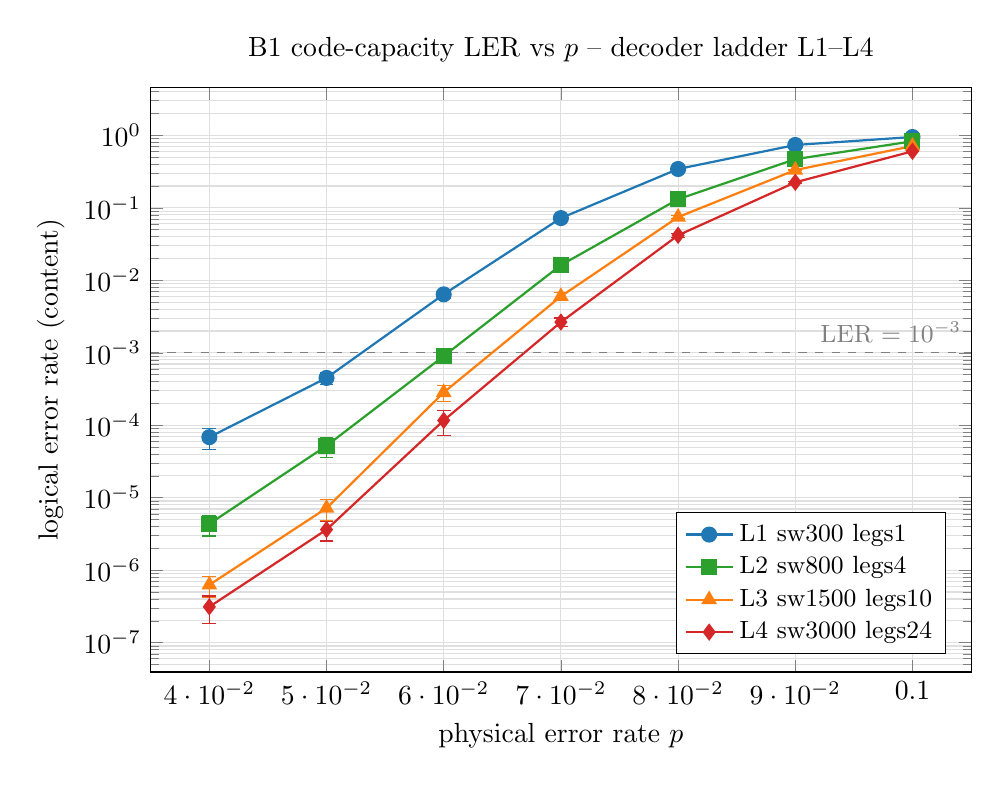
\begin{tikzpicture}
\begin{semilogyaxis}[
    width=12cm, height=9cm,
    xlabel={physical error rate $p$},
    ylabel={logical error rate (content)},
    title={B1 code-capacity LER vs $p$ -- decoder ladder L1--L4},
    xmin=0.035, xmax=0.105,
    xtick={0.04,0.05,0.06,0.07,0.08,0.09,0.1},
    grid=both, grid style={gray!25},
    legend pos=south east, legend cell align={left},
    legend style={font=\small},
    every axis plot/.append style={thick, mark options={solid}},
]
\addplot[color={rgb,255:red,31;green,119;blue,180}, mark=*, mark size=2.5pt,
    error bars/.cd, y dir=both, y explicit]
  coordinates {
    (0.04, 6.8490e-05) +- (0, 2.2000e-05)
    (0.05, 4.5000e-04) +- (0, 8.6603e-05)
    (0.06, 6.4000e-03) +- (0, 8.0000e-04)
    (0.07, 7.2200e-02) +- (0, 3.8000e-03)
    (0.08, 3.4340e-01) +- (0, 8.2873e-03)
    (0.09, 7.3660e-01) +- (0, 1.2138e-02)
    (0.1, 9.4880e-01) +- (0, 1.3775e-02)
  };
\addlegendentry{L1  sw300  legs1}
\addplot[color={rgb,255:red,44;green,160;blue,44}, mark=square*, mark size=2.5pt,
    error bars/.cd, y dir=both, y explicit]
  coordinates {
    (0.04, 4.3590e-06) +- (0, 1.4000e-06)
    (0.05, 5.2080e-05) +- (0, 1.6000e-05)
    (0.06, 9.0000e-04) +- (0, 1.5000e-04)
    (0.07, 1.6200e-02) +- (0, 1.8000e-03)
    (0.08, 1.3140e-01) +- (0, 5.1264e-03)
    (0.09, 4.6940e-01) +- (0, 9.6892e-03)
    (0.1, 8.2840e-01) +- (0, 1.2872e-02)
  };
\addlegendentry{L2  sw800  legs4}
\addplot[color={rgb,255:red,255;green,127;blue,14}, mark=triangle*, mark size=2.5pt,
    error bars/.cd, y dir=both, y explicit]
  coordinates {
    (0.04, 6.2740e-07) +- (0, 2.0000e-07)
    (0.05, 7.1840e-06) +- (0, 2.3000e-06)
    (0.06, 2.8333e-04) +- (0, 6.8718e-05)
    (0.07, 6.0000e-03) +- (0, 7.7460e-04)
    (0.08, 7.4600e-02) +- (0, 3.8626e-03)
    (0.09, 3.3200e-01) +- (0, 8.1486e-03)
    (0.1, 7.1240e-01) +- (0, 1.1936e-02)
  };
\addlegendentry{L3  sw1500 legs10}
\addplot[color={rgb,255:red,214;green,39;blue,40}, mark=diamond*, mark size=2.5pt,
    error bars/.cd, y dir=both, y explicit]
  coordinates {
    (0.04, 3.1247e-07) +- (0, 1.2756e-07)
    (0.05, 3.6310e-06) +- (0, 1.1000e-06)
    (0.06, 1.1667e-04) +- (0, 4.4096e-05)
    (0.07, 2.6500e-03) +- (0, 3.6401e-04)
    (0.08, 4.1800e-02) +- (0, 2.8914e-03)
    (0.09, 2.2480e-01) +- (0, 6.7052e-03)
    (0.1, 6.0280e-01) +- (0, 1.0980e-02)
  };
\addlegendentry{L4  sw3000 legs24}
\draw[dashed, gray] (axis cs:0.035,1e-3) -- (axis cs:0.105,1e-3);
\node[gray, font=\small, anchor=south east] at (axis cs:0.105,1e-3)
    {LER $=10^{-3}$};
\end{semilogyaxis}
\end{tikzpicture}
\end{document}
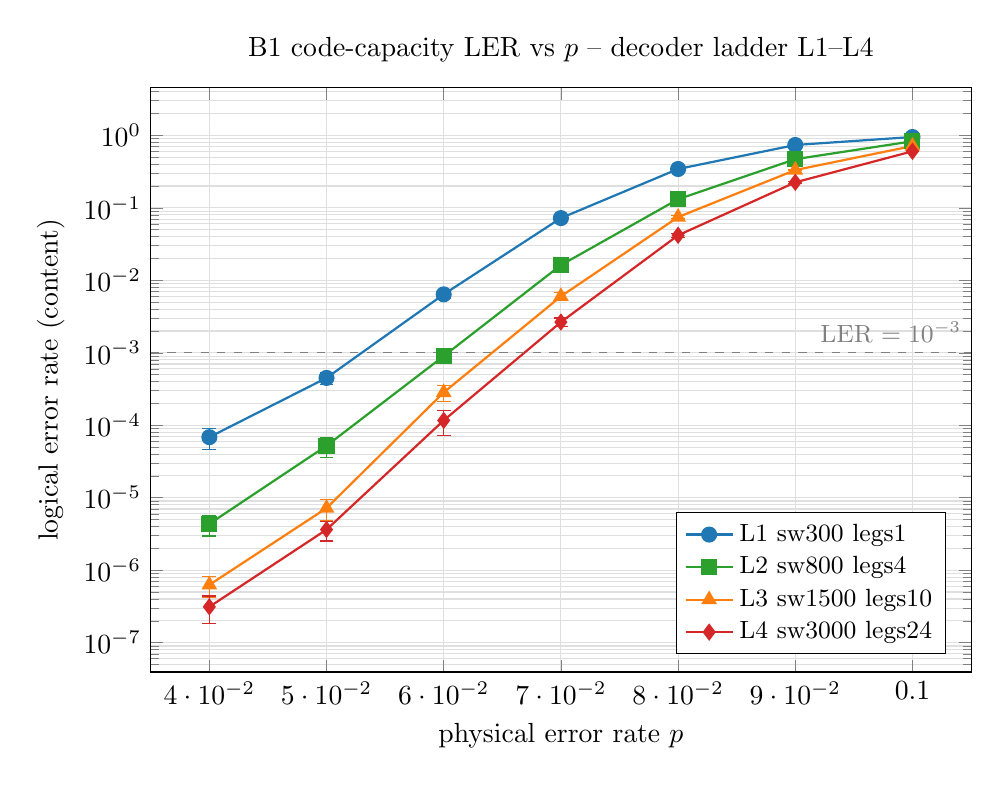
\begin{tikzpicture}
\begin{semilogyaxis}[
    width=12cm, height=9cm,
    xlabel={physical error rate $p$},
    ylabel={logical error rate (content)},
    title={B1 code-capacity LER vs $p$ -- decoder ladder L1--L4},
    xmin=0.035, xmax=0.105,
    xtick={0.04,0.05,0.06,0.07,0.08,0.09,0.1},
    grid=both, grid style={gray!25},
    legend pos=south east, legend cell align={left},
    legend style={font=\small},
    every axis plot/.append style={thick, mark options={solid}},
]
\addplot[color={rgb,255:red,31;green,119;blue,180}, mark=*, mark size=2.5pt,
    error bars/.cd, y dir=both, y explicit]
  coordinates {
    (0.04, 6.8490e-05) +- (0, 2.2000e-05)
    (0.05, 4.5000e-04) +- (0, 8.6603e-05)
    (0.06, 6.4000e-03) +- (0, 8.0000e-04)
    (0.07, 7.2200e-02) +- (0, 3.8000e-03)
    (0.08, 3.4340e-01) +- (0, 8.2873e-03)
    (0.09, 7.3660e-01) +- (0, 1.2138e-02)
    (0.1, 9.4880e-01) +- (0, 1.3775e-02)
  };
\addlegendentry{L1  sw300  legs1}
\addplot[color={rgb,255:red,44;green,160;blue,44}, mark=square*, mark size=2.5pt,
    error bars/.cd, y dir=both, y explicit]
  coordinates {
    (0.04, 4.3590e-06) +- (0, 1.4000e-06)
    (0.05, 5.2080e-05) +- (0, 1.6000e-05)
    (0.06, 9.0000e-04) +- (0, 1.5000e-04)
    (0.07, 1.6200e-02) +- (0, 1.8000e-03)
    (0.08, 1.3140e-01) +- (0, 5.1264e-03)
    (0.09, 4.6940e-01) +- (0, 9.6892e-03)
    (0.1, 8.2840e-01) +- (0, 1.2872e-02)
  };
\addlegendentry{L2  sw800  legs4}
\addplot[color={rgb,255:red,255;green,127;blue,14}, mark=triangle*, mark size=2.5pt,
    error bars/.cd, y dir=both, y explicit]
  coordinates {
    (0.04, 6.2740e-07) +- (0, 2.0000e-07)
    (0.05, 7.1840e-06) +- (0, 2.3000e-06)
    (0.06, 2.8333e-04) +- (0, 6.8718e-05)
    (0.07, 6.0000e-03) +- (0, 7.7460e-04)
    (0.08, 7.4600e-02) +- (0, 3.8626e-03)
    (0.09, 3.3200e-01) +- (0, 8.1486e-03)
    (0.1, 7.1240e-01) +- (0, 1.1936e-02)
  };
\addlegendentry{L3  sw1500 legs10}
\addplot[color={rgb,255:red,214;green,39;blue,40}, mark=diamond*, mark size=2.5pt,
    error bars/.cd, y dir=both, y explicit]
  coordinates {
    (0.04, 3.1247e-07) +- (0, 1.2756e-07)
    (0.05, 3.6310e-06) +- (0, 1.1000e-06)
    (0.06, 1.1667e-04) +- (0, 4.4096e-05)
    (0.07, 2.6500e-03) +- (0, 3.6401e-04)
    (0.08, 4.1800e-02) +- (0, 2.8914e-03)
    (0.09, 2.2480e-01) +- (0, 6.7052e-03)
    (0.1, 6.0280e-01) +- (0, 1.0980e-02)
  };
\addlegendentry{L4  sw3000 legs24}
\draw[dashed, gray] (axis cs:0.035,1e-3) -- (axis cs:0.105,1e-3);
\node[gray, font=\small, anchor=south east] at (axis cs:0.105,1e-3)
    {LER $=10^{-3}$};
\end{semilogyaxis}
\end{tikzpicture}
\end{document}
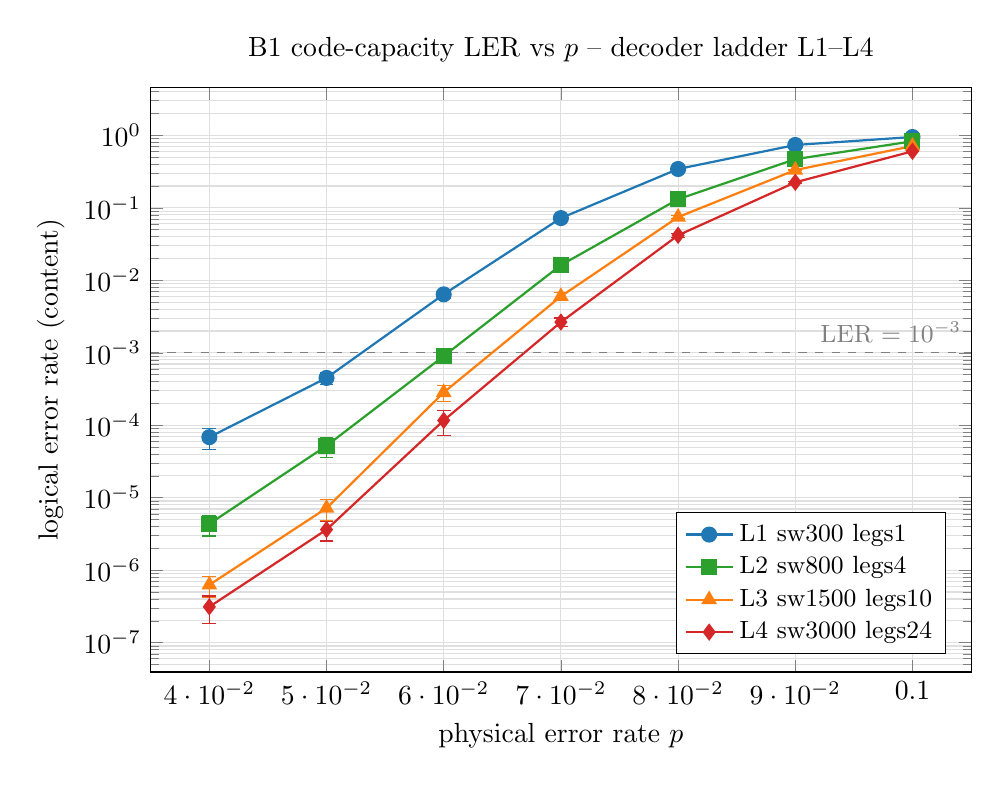
\begin{tikzpicture}
\begin{semilogyaxis}[
    width=12cm, height=9cm,
    xlabel={physical error rate $p$},
    ylabel={logical error rate (content)},
    title={B1 code-capacity LER vs $p$ -- decoder ladder L1--L4},
    xmin=0.035, xmax=0.105,
    xtick={0.04,0.05,0.06,0.07,0.08,0.09,0.1},
    grid=both, grid style={gray!25},
    legend pos=south east, legend cell align={left},
    legend style={font=\small},
    every axis plot/.append style={thick, mark options={solid}},
]
\addplot[color={rgb,255:red,31;green,119;blue,180}, mark=*, mark size=2.5pt,
    error bars/.cd, y dir=both, y explicit]
  coordinates {
    (0.04, 6.8490e-05) +- (0, 2.2000e-05)
    (0.05, 4.5000e-04) +- (0, 8.6603e-05)
    (0.06, 6.4000e-03) +- (0, 8.0000e-04)
    (0.07, 7.2200e-02) +- (0, 3.8000e-03)
    (0.08, 3.4340e-01) +- (0, 8.2873e-03)
    (0.09, 7.3660e-01) +- (0, 1.2138e-02)
    (0.1, 9.4880e-01) +- (0, 1.3775e-02)
  };
\addlegendentry{L1  sw300  legs1}
\addplot[color={rgb,255:red,44;green,160;blue,44}, mark=square*, mark size=2.5pt,
    error bars/.cd, y dir=both, y explicit]
  coordinates {
    (0.04, 4.3590e-06) +- (0, 1.4000e-06)
    (0.05, 5.2080e-05) +- (0, 1.6000e-05)
    (0.06, 9.0000e-04) +- (0, 1.5000e-04)
    (0.07, 1.6200e-02) +- (0, 1.8000e-03)
    (0.08, 1.3140e-01) +- (0, 5.1264e-03)
    (0.09, 4.6940e-01) +- (0, 9.6892e-03)
    (0.1, 8.2840e-01) +- (0, 1.2872e-02)
  };
\addlegendentry{L2  sw800  legs4}
\addplot[color={rgb,255:red,255;green,127;blue,14}, mark=triangle*, mark size=2.5pt,
    error bars/.cd, y dir=both, y explicit]
  coordinates {
    (0.04, 6.2740e-07) +- (0, 2.0000e-07)
    (0.05, 7.1840e-06) +- (0, 2.3000e-06)
    (0.06, 2.8333e-04) +- (0, 6.8718e-05)
    (0.07, 6.0000e-03) +- (0, 7.7460e-04)
    (0.08, 7.4600e-02) +- (0, 3.8626e-03)
    (0.09, 3.3200e-01) +- (0, 8.1486e-03)
    (0.1, 7.1240e-01) +- (0, 1.1936e-02)
  };
\addlegendentry{L3  sw1500 legs10}
\addplot[color={rgb,255:red,214;green,39;blue,40}, mark=diamond*, mark size=2.5pt,
    error bars/.cd, y dir=both, y explicit]
  coordinates {
    (0.04, 3.1247e-07) +- (0, 1.2756e-07)
    (0.05, 3.6310e-06) +- (0, 1.1000e-06)
    (0.06, 1.1667e-04) +- (0, 4.4096e-05)
    (0.07, 2.6500e-03) +- (0, 3.6401e-04)
    (0.08, 4.1800e-02) +- (0, 2.8914e-03)
    (0.09, 2.2480e-01) +- (0, 6.7052e-03)
    (0.1, 6.0280e-01) +- (0, 1.0980e-02)
  };
\addlegendentry{L4  sw3000 legs24}
\draw[dashed, gray] (axis cs:0.035,1e-3) -- (axis cs:0.105,1e-3);
\node[gray, font=\small, anchor=south east] at (axis cs:0.105,1e-3)
    {LER $=10^{-3}$};
\end{semilogyaxis}
\end{tikzpicture}
